%%%%%%%%%%%%%%%%%%%%%%%%%%%%%%%%%%%%%%%%%%%%%%%%%%%
\fe{\section{Présentation}}{\section{Presentation}}
\label{presentation}
%%%%%%%%%%%%%%%%%%%%%%%%%%%%%%%%%%%%%%%%%%%%%%%%%%%

\begin{frame}{\fe{Cast3M, quid ?}{What is Cast3M?}}
  \begin{center}
  \fe{Logiciel de simulation utilisant la \g{méthode des éléments finis} en \g{mécanique/thermique} des \g{structures} et des \g{fluides}}
     {A simulation software using the \g{finite element method} in \g{thermal and mechanical} analysis of \g{structures} and \g{fluids}}\pause
  \end{center}
  \begin{itemize}
    \item \fe{Résolution d'\g{équations aux dérivées partielles}}
             {\g{Partial differential equations} solver}\pause
    \item \fe{\g{Système complet} : solveur, pré/post-processeur, visualisation, import/export des données\dots}
             {\g{Complete software}: solver, pre-processing and post-processing, visualization, reading/writing data\dots}\\
            ~\\
            \begin{center}
            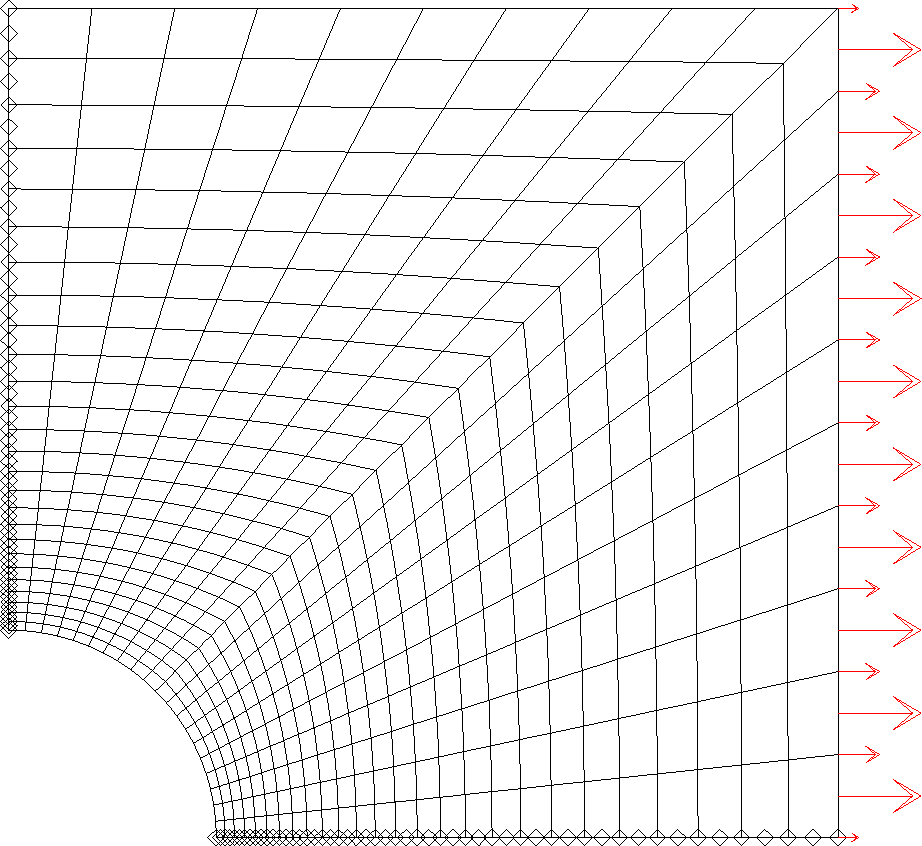
\includegraphics[height=0.25\textheight]{images/plaque.1} \:
            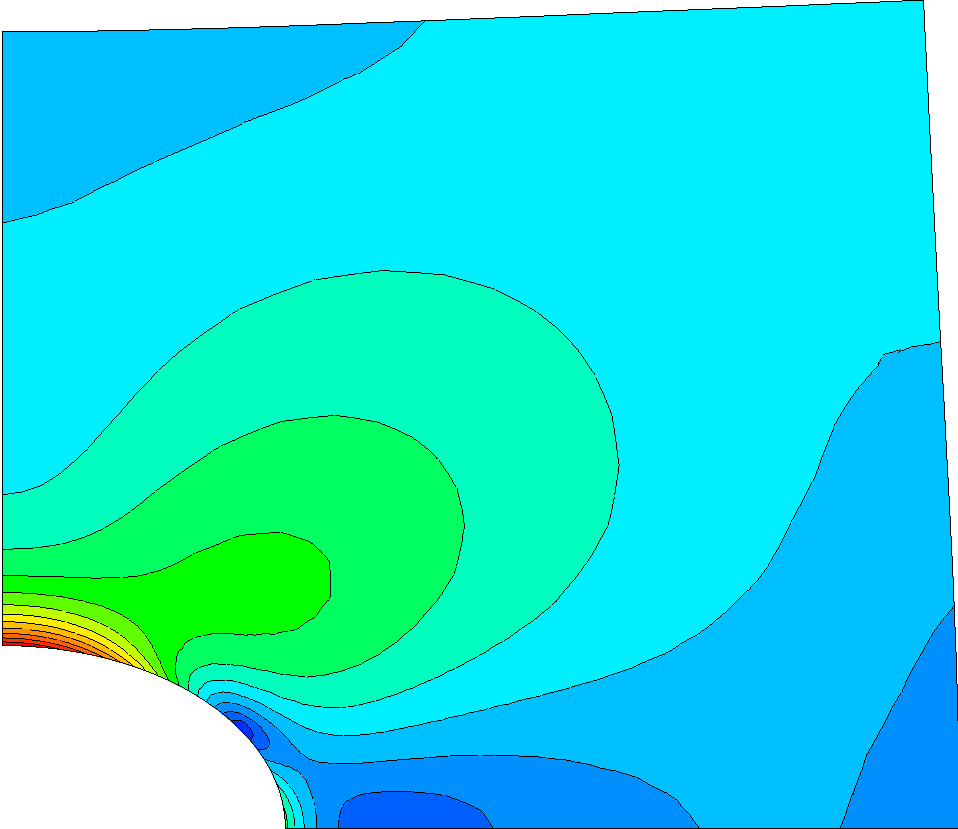
\includegraphics[height=0.25\textheight]{images/plaque.2} \:
            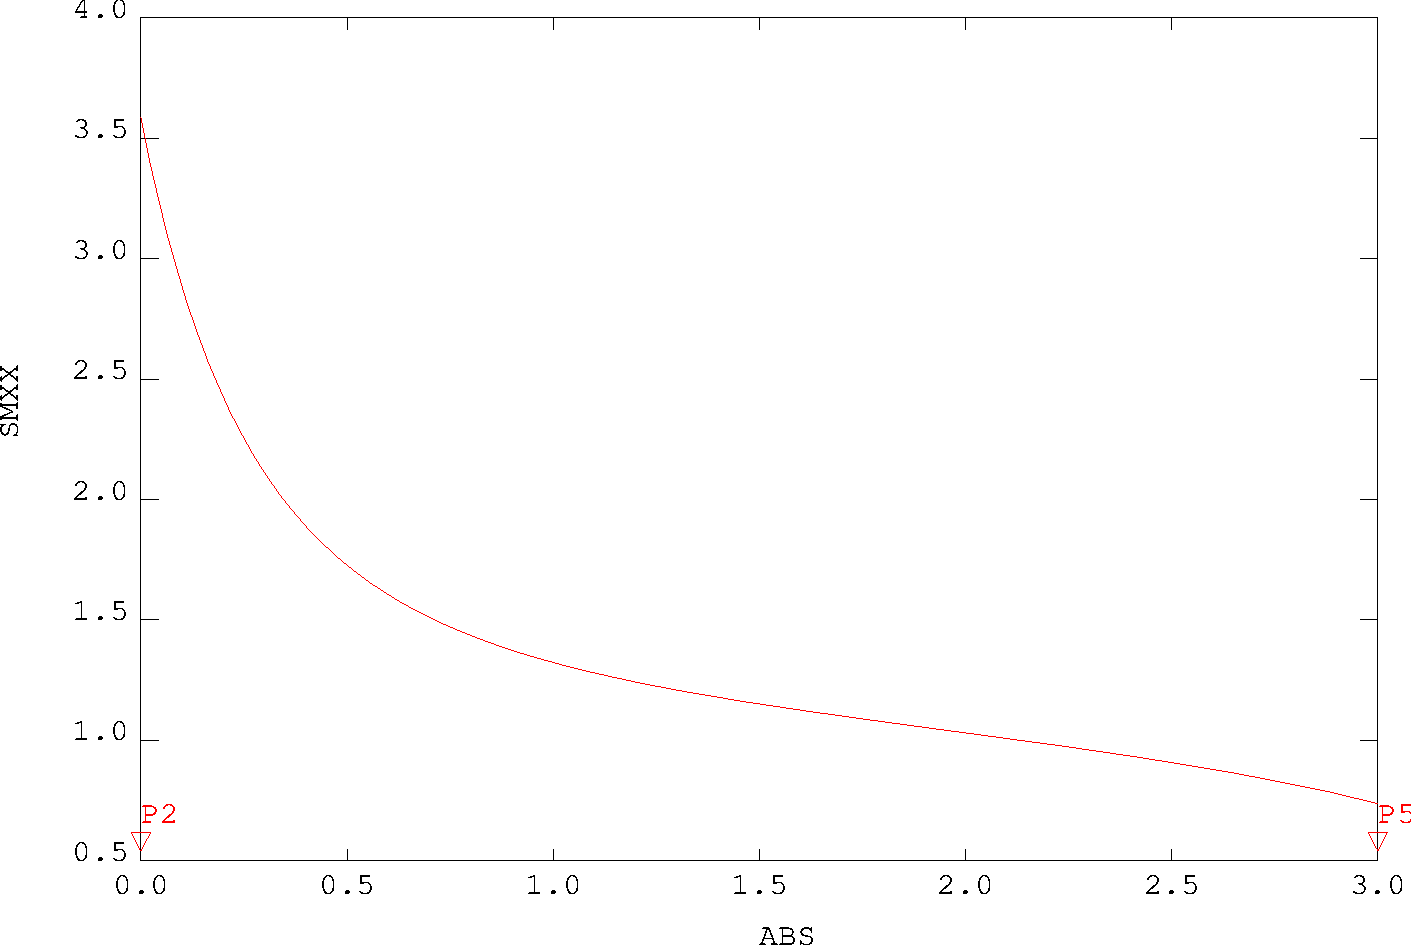
\includegraphics[height=0.25\textheight]{images/plaque.3}
            \end{center}\pause
    \item \fe{Basé sur un langage de commande : \g{Gibiane} (orienté objet)}
             {Based on a programming language: \g{Gibiane} (objet-oriented)}\\
  \end{itemize}
\end{frame}

\begin{frame}{\fe{Nombreux domaines d'application}{Wide range of applications}}
  \small{
  \begin{itemize}
    \item<1->\fe{Mécanique des structures}{Structural mechanics}\\
    \footnotesize{
      \fe{\red{Quasi-statique} (non linéarités matériau, géométrie, conditions limites)}
         {\red{Quasi-static} (non linear behavior, geometry, boundary conditions)}\\
      \onslide<1>{
        \begin{textblock*}{5cm}(2cm,0.3cm)
          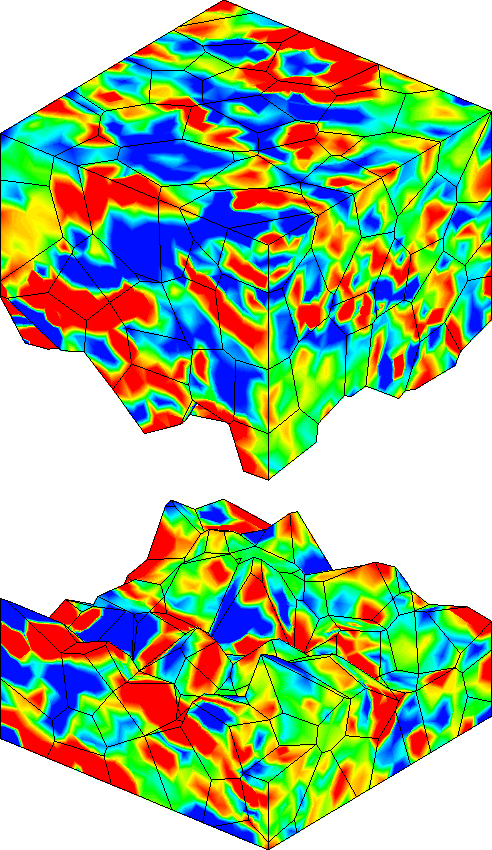
\includegraphics[height=0.4\textheight]{images/polycristal}
        \end{textblock*}
        \begin{textblock*}{5cm}(5cm,1.2cm)
          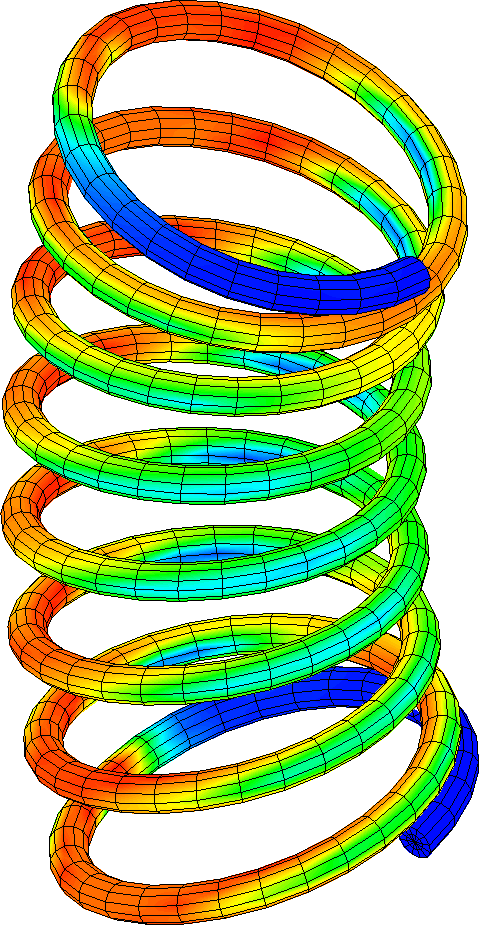
\includegraphics[height=0.4\textheight]{images/ressort}
        \end{textblock*}
        \begin{textblock*}{5cm}(8cm,2.1cm)
          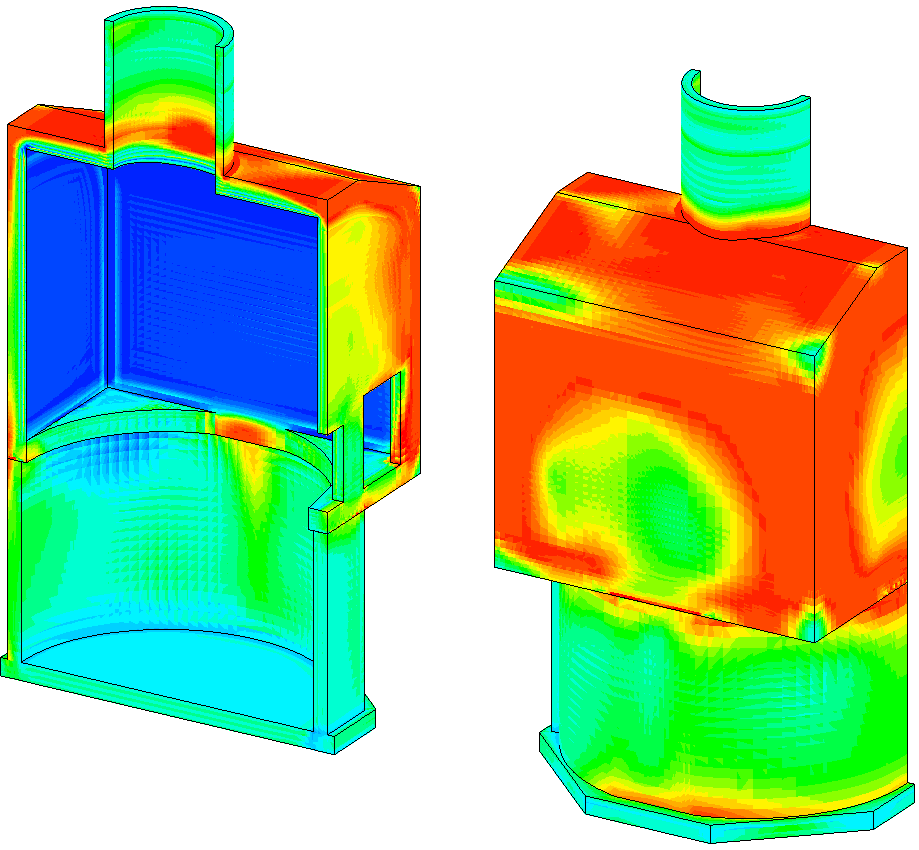
\includegraphics[height=0.4\textheight]{images/galatee}
        \end{textblock*}
        \begin{textblock*}{5cm}(9.4cm,5.6cm)
          \tiny{\emph{(S. Durand)}}
        \end{textblock*}}
      \onslide<2->\fe{\orange{Contact/frottement}, \green{Flambage}}
                     {\orange{Contact/friction}, \green{Buckling}}\\
      \onslide<2>{
        \begin{textblock*}{5cm}(1cm,0.3cm)
          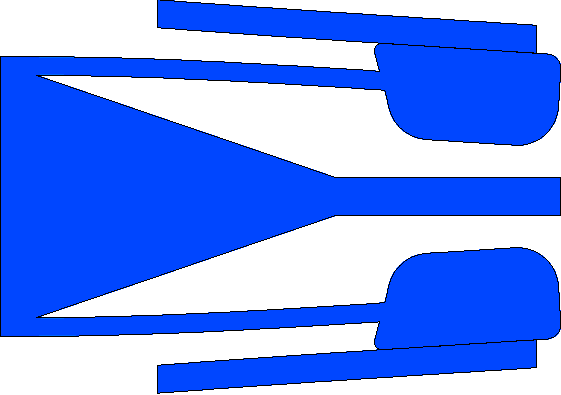
\includegraphics[height=0.25\textheight]{images/sac_a_dos.15}
        \end{textblock*}
        \begin{textblock*}{5cm}(4.8cm,0.3cm)
          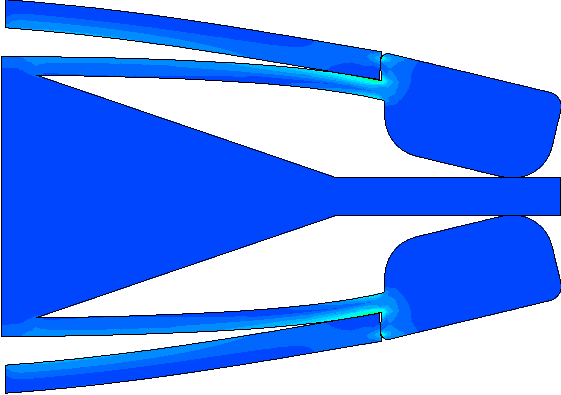
\includegraphics[height=0.25\textheight]{images/sac_a_dos.32}
        \end{textblock*}
        \begin{textblock*}{5cm}(8.5cm,0.3cm)
          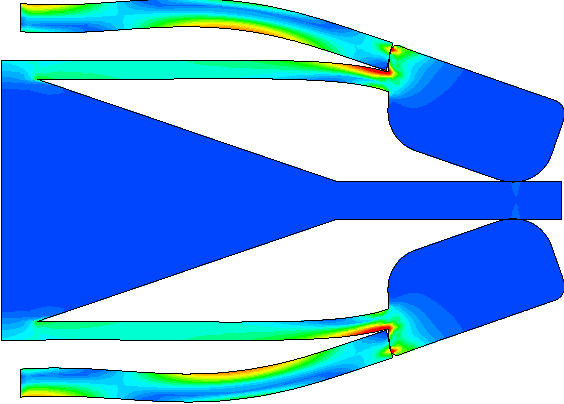
\includegraphics[height=0.25\textheight]{images/sac_a_dos.41}
        \end{textblock*}}
      \onslide<3->\fe{\blue{Dynamique} (temporelle, modale, interaction fluide structure)}
                     {\blue{Dynamic} (temporal, modal, fluid structure interaction)}\\
      \onslide<3>{
        \begin{textblock*}{5cm}(1cm,0.3cm)
          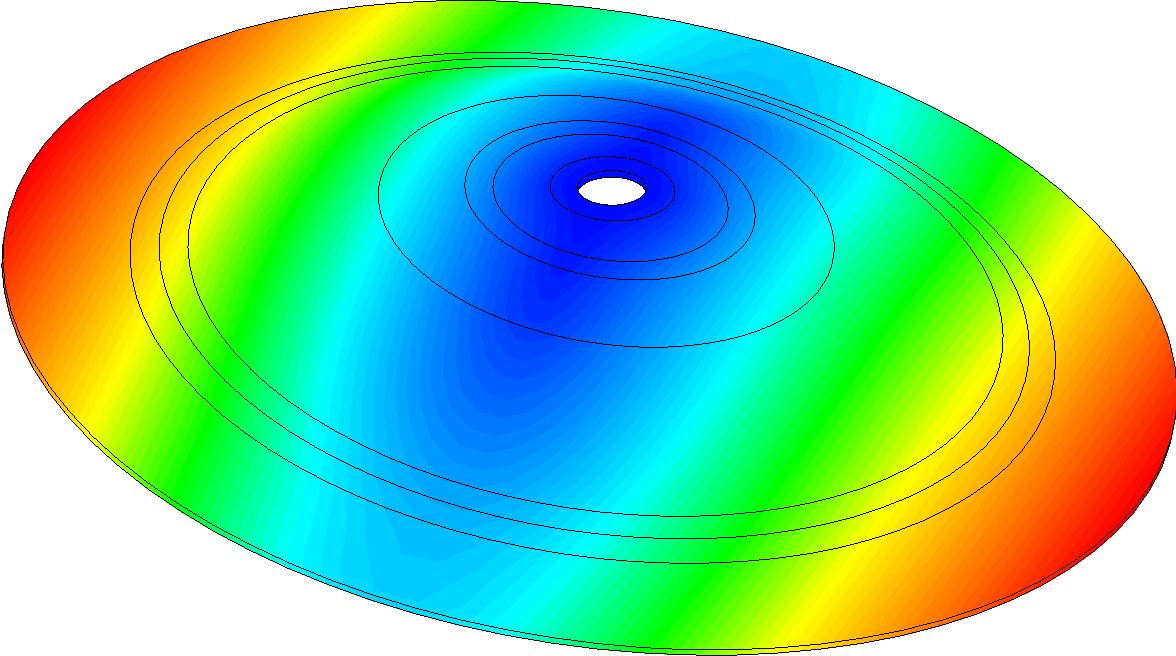
\includegraphics[height=0.2\textheight]{images/cymbale_mode_1}
        \end{textblock*}
        \begin{textblock*}{5cm}(4.8cm,0.3cm)
          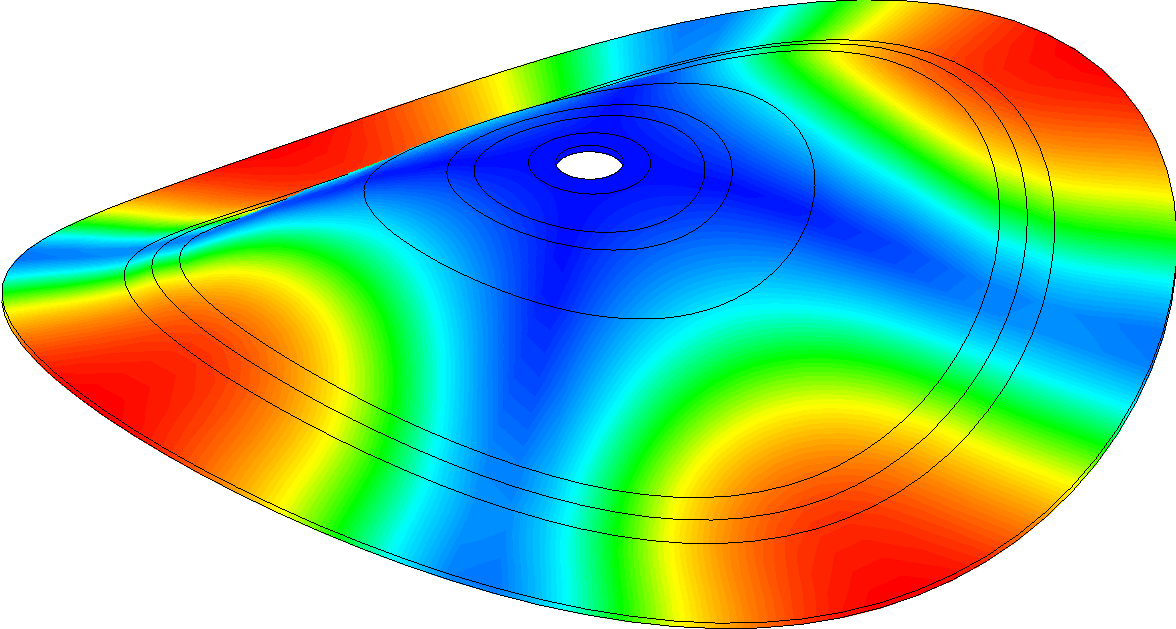
\includegraphics[height=0.2\textheight]{images/cymbale_mode_2}
        \end{textblock*}
        \begin{textblock*}{5cm}(8.5cm,0.3cm)
          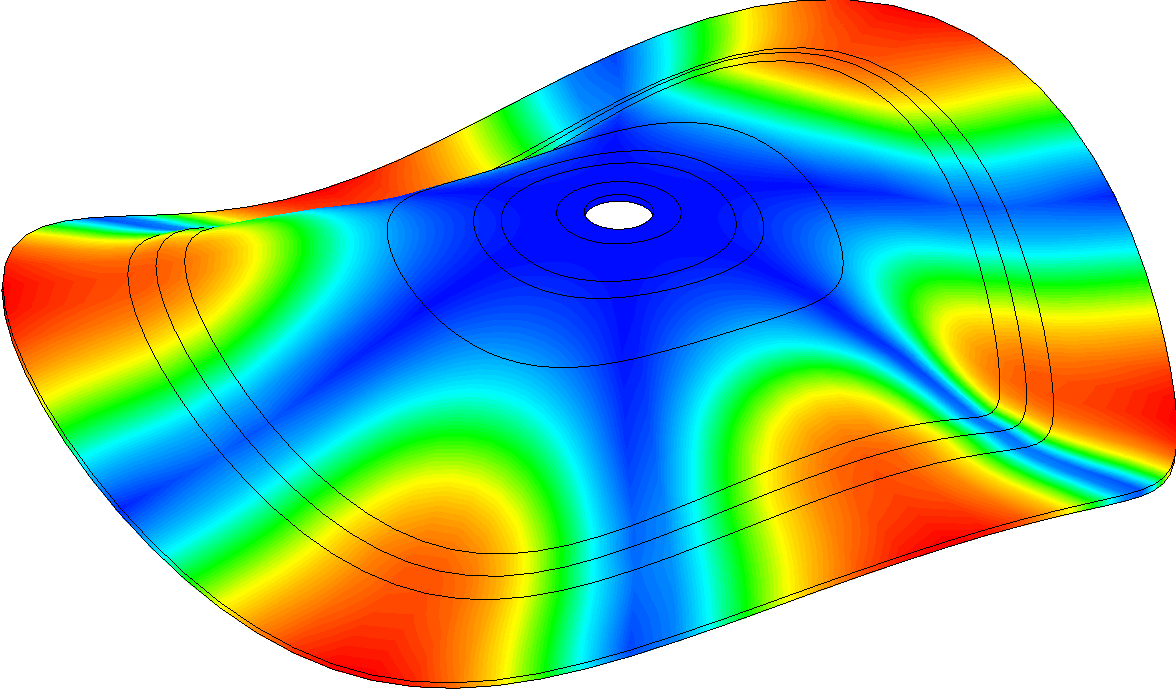
\includegraphics[height=0.2\textheight]{images/cymbale_mode_4}
        \end{textblock*}}
      \onslide<4->\fe{\violet{Rupture} (XFEM, propagation dynamique, zones cohésives)}
                     {\violet{Fracture} (XFEM, dynamic propagation, cohesive zones models)}\\
      \onslide<4>{
        \begin{textblock*}{12cm}(1.5cm,0.3cm)
          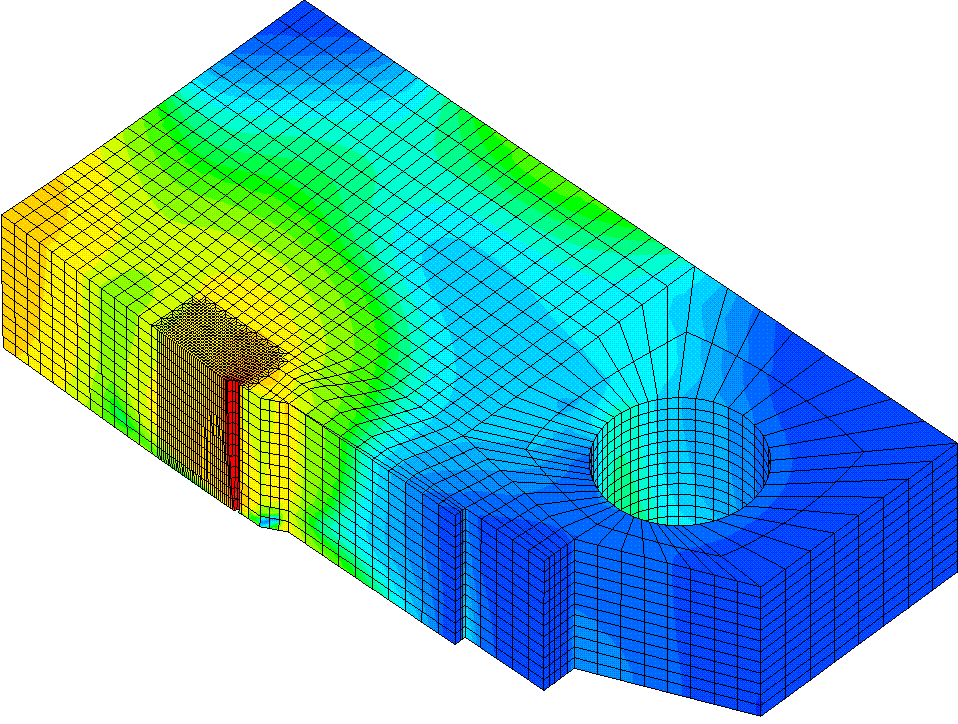
\includegraphics[height=0.25\textheight]{images/rousselier_03}
          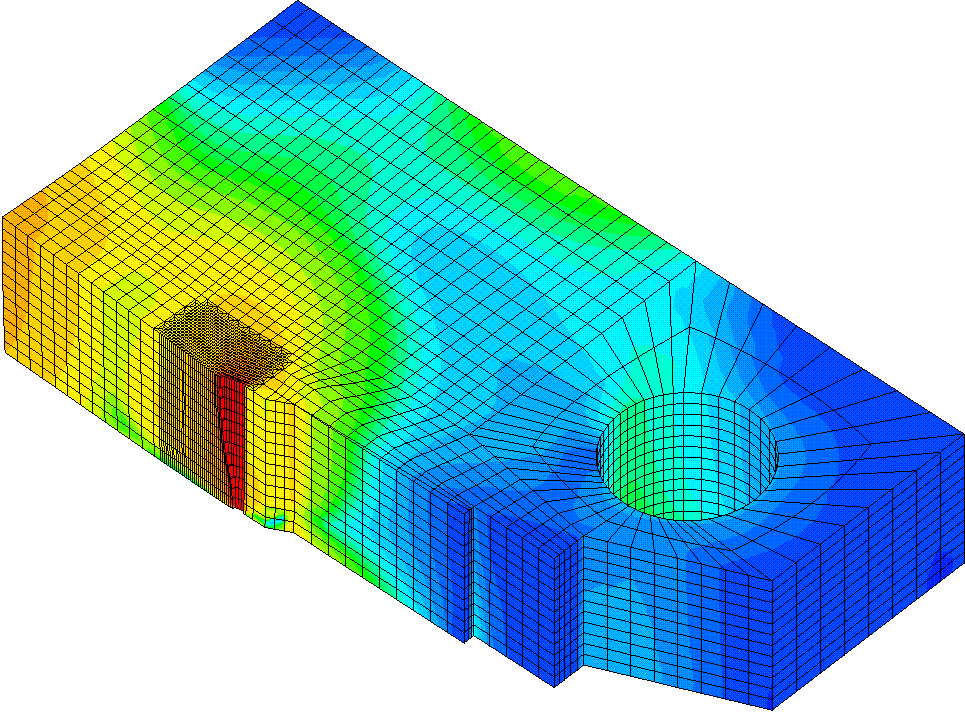
\includegraphics[height=0.25\textheight]{images/rousselier_04}
          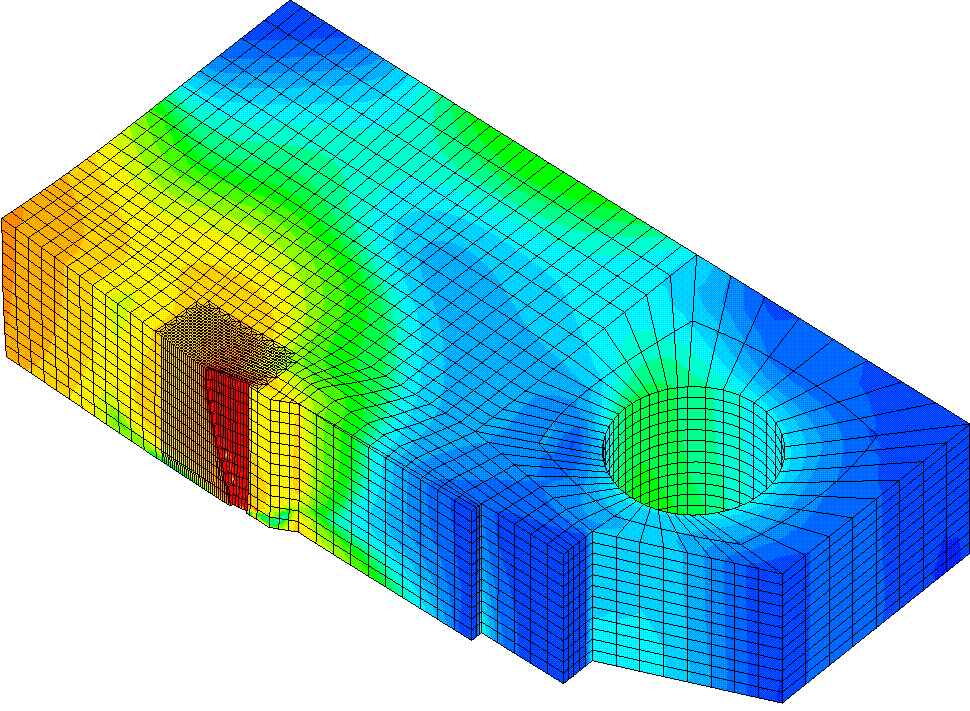
\includegraphics[height=0.25\textheight]{images/rousselier_05}
          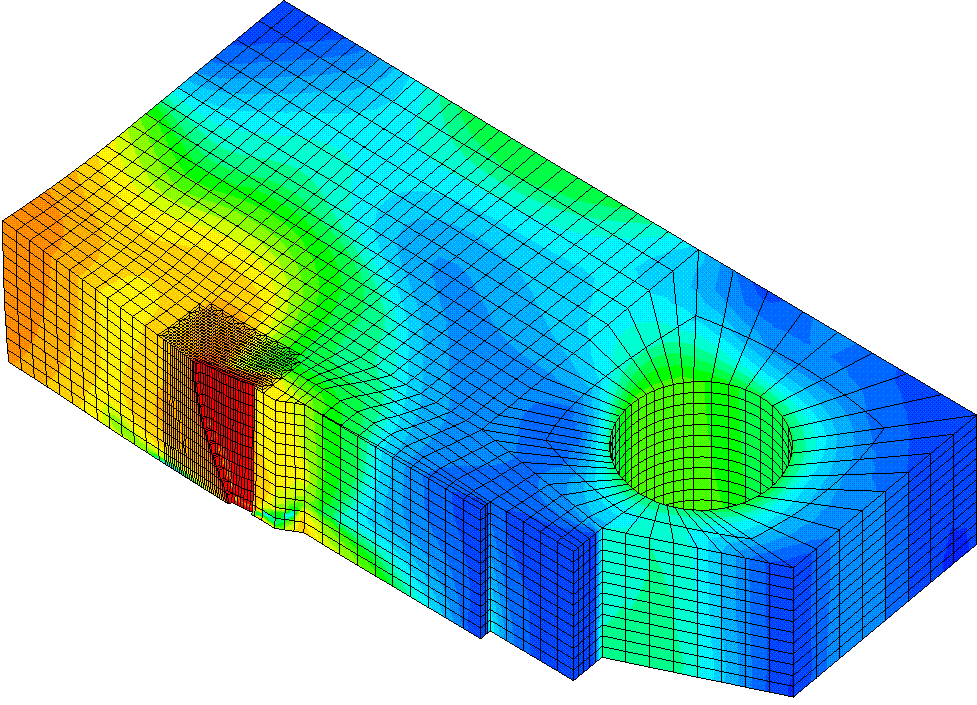
\includegraphics[height=0.25\textheight]{images/rousselier_06}
          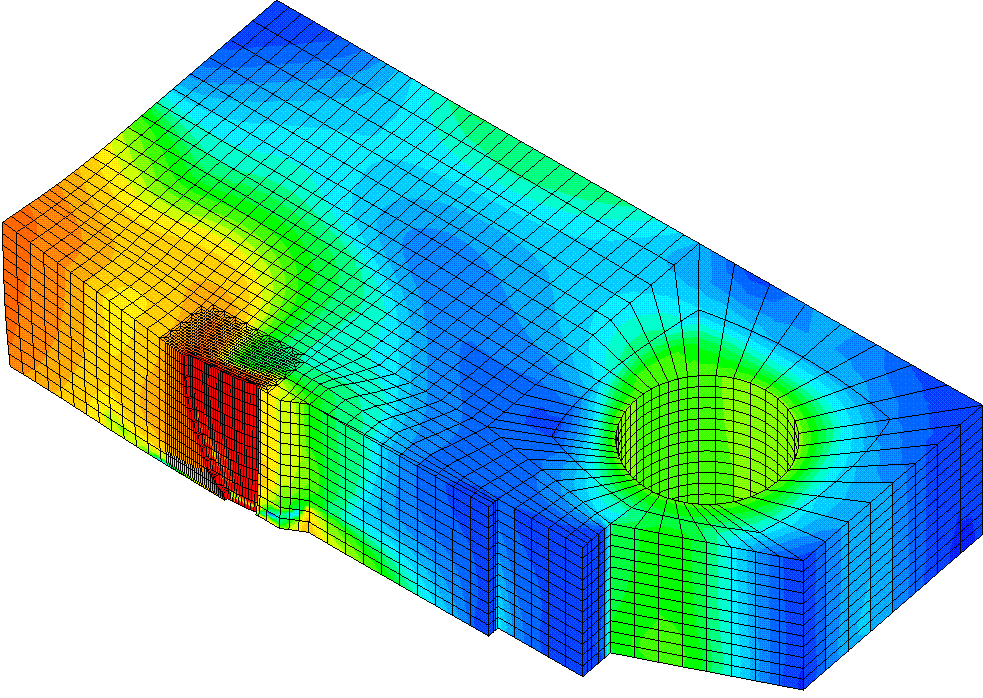
\includegraphics[height=0.25\textheight]{images/rousselier_07}
          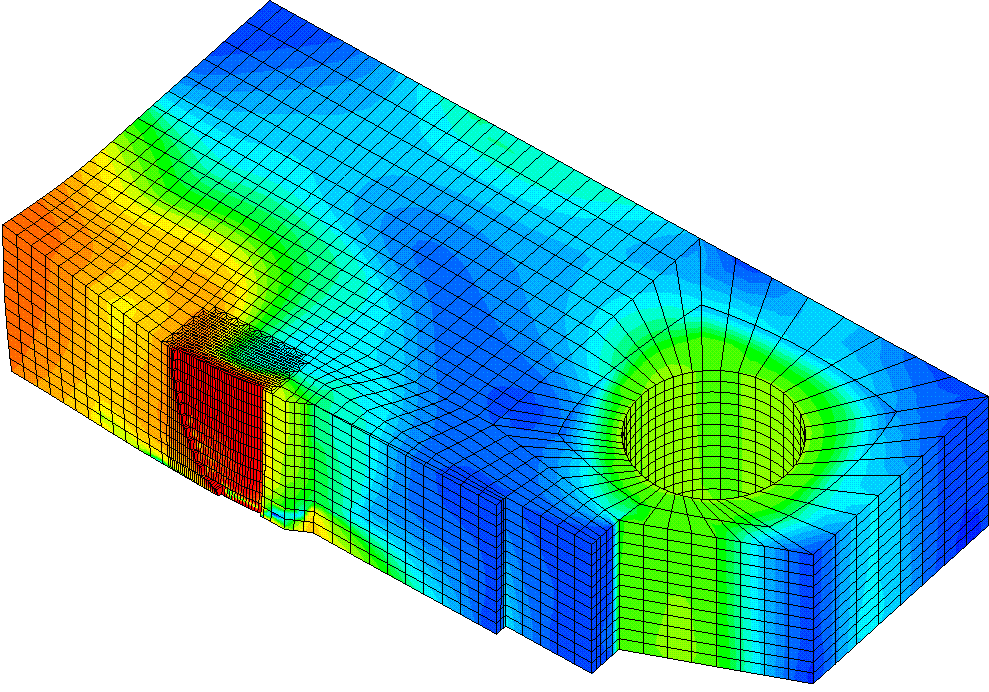
\includegraphics[height=0.25\textheight]{images/rousselier_08}
        \end{textblock*}
        \begin{textblock*}{5cm}(8cm,4.7cm)
          \tiny{\emph{(S. Kebiri)}}
        \end{textblock*}}
      \onslide<5>{
        \begin{textblock*}{12cm}(3.5cm,1.3cm)
          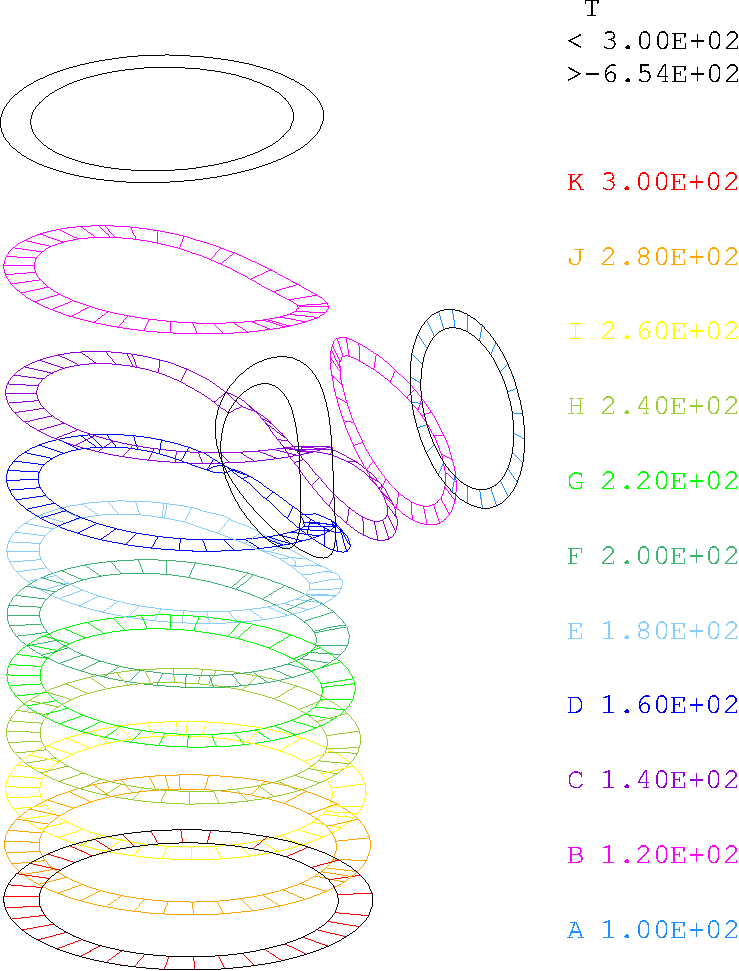
\includegraphics[height=0.4\textheight]{images/te_temperature}\hspace{1cm}
          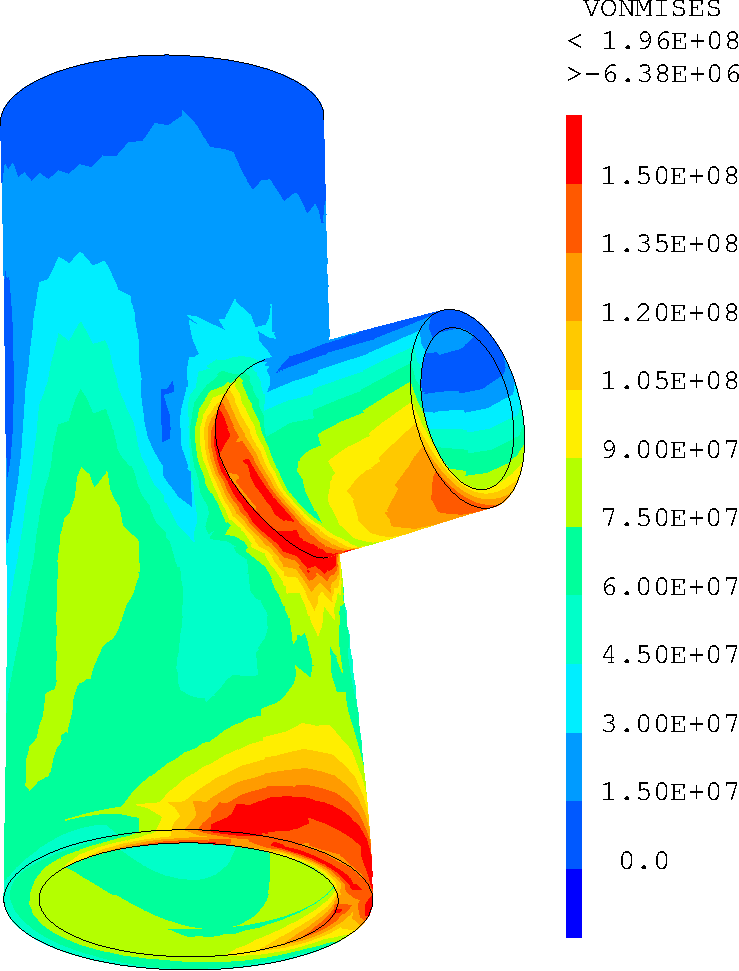
\includegraphics[height=0.4\textheight]{images/te_sigma}
        \end{textblock*}}
      \onslide<6>{
        \begin{textblock*}{12cm}(6.5cm,1.2cm)
          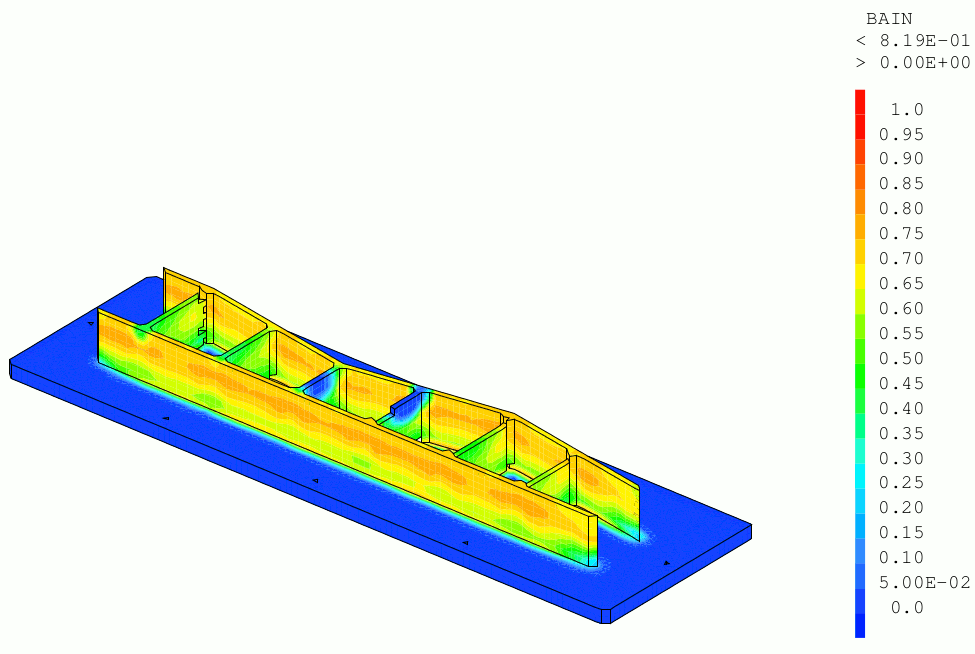
\includegraphics[height=0.4\textheight]{images/metallurgie}
        \end{textblock*}
        \begin{textblock*}{5cm}(8cm,4.7cm)
          \tiny{\emph{(C. Berthinier)}}
        \end{textblock*}}
    }
    \item<5->\fe{Thermique}{Thermal analysis}\\
    \footnotesize{
      \fe{Conduction, convection, rayonnement, changement de phase}
         {Conduction, convection, radiation, phase transition}
    }
    \item<6->\fe{Mécanique des fluides}{Fluid mechanics}
    \item<6->\fe{Magnétostatique}{Magneto-statics}
    \item<6->\fe{Diffusion multi espèces (loi de Fick)}{Multi species diffusion (Fick’s law)}
    \item<6->\fe{Métallurgie}{Metallurgy}
  \item<6->\fe{Couplage thermo-hygro-mécanique}{Thermo-hygro-mechanics coupling}
  \end{itemize}
  }
\end{frame}

\begin{frame}{\fe{Comment obtenir Cast3M ?}{How to get Cast3M}}
  \begin{itemize}
    \item \fe{Multi plateformes}{Cross platform}\\
    \footnotesize
    \blue{Windows}, \red{Linux}, \green{macOS}
    \normalsize
    \item \fe{Où télécharger Cast3M ?}{Where can I download Cast3M?}\\
    \footnotesize
    \url{http://www-cast3m.cea.fr/index.php?page=dlcastem}
    \normalsize
    \item \fe{Accès au code source}{Access to the source code}\\
    \footnotesize
    \fe{Développement communautaire}{Open collaboration}\\
    \fe{Compilateur / éditeur de liens fournis}{Compiler / Linker are provided}
    \normalsize
    \item \fe{Prix}{Price}\\
    \footnotesize
    \fe{\green{Gratuit} pour la recherche et l’enseignement\\
        \red{Payant} pour une utilisation commerciale}
       {\green{Free} license, for education and research use\\
        \red{Paid} license, for enterprise use}
    \normalsize
    \item \fe{Utilisateurs/clients}{Users/customers}\\
    \footnotesize
    \fe{Universités, écoles d’ingénieurs\\
        IRSN, EDF, SNCF, CNRS, Framatome, Air Liquide, CERN, \dots}
       {Universities, engineering schools\\
        IRSN, EDF, SNCF, CNRS, Framatome, Air Liquide, CERN, \dots}\\
    \scriptsize
    \fe{Outil de référence IRSN pour les analyse de sureté des installations nucléaires françaises\\
        Outil de référence Framatome pour l’analyse en mécanique de la rupture}
       {Reference FEM tool for IRSN for safety analysis of French nuclear installations\\
        Reference tool for Framatome for fracture mechanics}
    \normalsize
    \end{itemize}
\end{frame}

\begin{frame}{\fe{Comment utiliser Cast3M ?}{How to launch Cast3M?}}
  \begin{textblock*}{5cm}(7.9cm,0cm)
    \animategraphics[autoplay,loop,poster=last,width=4.5cm]{10}{images/new_dgibi/new_dgibi-}{000}{235}
  \end{textblock*}
  \begin{enumerate}
    \item\fe{Écrire un fichier texte en Gibiane}{Write a Gibiane script in a text file}\\
    \footnotesize
    \fe{et l'enregistrer dans un répertoire de travail}{and save it in a working directory}
    \normalsize
    \item[]\white{O/}\\
    \footnotesize
    \white{et}\\
    \normalsize
    \item[]\white{Cast3M}\\
    \footnotesize
    \white{castem24  hello.dgibi}
    \normalsize
    \item[]\white{U}\\
    \footnotesize
    \white{mode}\\
    \white{castem24}
    \normalsize
  \end{enumerate}
\end{frame}

\begin{frame}{\fe{Comment utiliser Cast3M ?}{How to launch Cast3M?}}
  \begin{textblock*}{5cm}(7.9cm,0cm)
    \animategraphics[autoplay,loop,poster=last,width=4.5cm]{10}{images/new_cmd/new_cmd-}{000}{179}
  \end{textblock*}
  \begin{enumerate}
    \item\fe{Écrire un fichier texte en Gibiane}{Write a Gibiane script in a text file}\\
    \footnotesize
    \fe{et l'enregistrer dans un répertoire de travail}{and save it in a working directory}
    \normalsize
    \item\fe{Ouvrir un terminal / invite de commandes}{Open a terminal / command prompt}\\
    \footnotesize
    \fe{et se placer dans le répertoire}{and go to the working directory}\\
    \normalsize
    \item\fe{Lancer Cast3M sur ce fichier}{Launch Cast3M on this file}\\
    \footnotesize
    \kw{castem24  hello.dgibi}
    \normalsize
    \item\fe{Utilisable aussi sans fichier}{Can also be use without file}\\
    \footnotesize
    \fe{mode interactif}{interactive mode}\\
    \kw{castem24}
    \normalsize
  \end{enumerate}
\end{frame}

\begin{frame}{\fe{Le site web Cast3M}{The Cast3M web site}}
  \begin{center}
    \url{http://www-cast3m.cea.fr/}
  \end{center}
  \begin{itemize}
    \item \fe{Présentation de Cast3M}{Cast3M presentation}
    \item \fe{Formation et tutoriels vidéo}{Training courses and video tutorials}
    \item \fe{Documentation (notices, manuels, sources, exemples)}{Documentation (manual pages, source code, examples)}
    \item \fe{Fiches d'anomalie et de développement}{Anomaly and development reports}
    \item \fe{Téléchargements}{Downloads}
    \item \fe{Contact : support Cast3M}{Contact: Cast3M support}
    \item \fe{Communauté : liste de diffusion, club Cast3M}{Community: mailing list, Cast3M club}
  \end{itemize}
\end{frame}
